\documentclass[11pt]{article}
\usepackage[margin=1in]{geometry}
\usepackage{amsmath,amssymb,amsthm,mathtools}
\usepackage{dsfont}
\usepackage{graphicx}
\usepackage{booktabs}
\usepackage{array}
\usepackage{multirow}
\usepackage{placeins}
\usepackage[hyphens]{url}
\usepackage{microtype}
\usepackage{xcolor}
\usepackage{caption}
\captionsetup{font=small,labelfont=bf,margin=0.5em}
\usepackage[colorlinks=true,linkcolor=blue!55!black,citecolor=blue!55!black,urlcolor=blue!55!black]{hyperref}

\newcommand{\Tr}{\operatorname{Tr}}
\newcommand{\Np}{N'}
\newcommand{\lp}{\ell'}
\newcommand{\one}{\mathds 1}
\newcommand{\ip}[2]{\langle #1,#2\rangle}
\newcommand{\PH}{P_{\!H}}
\newcommand{\Ex}{\mathrm{Ex}}
\newcommand{\Co}{\mathrm{Co}}

% status tags (as in the previous reports)
\definecolor{cest}{RGB}{30,90,160}
\definecolor{cder}{RGB}{20,120,70}
\definecolor{cnum}{RGB}{150,90,10}
\definecolor{cconj}{RGB}{160,40,40}
\newcommand{\tagbox}[2]{\textsf{\small\color{#1}[#2]}}
\newcommand{\EST}{\tagbox{cest}{literature}}
\newcommand{\DER}{\tagbox{cder}{derived}}
\newcommand{\VER}{\tagbox{cder}{derived + verified}}
\newcommand{\NUM}{\tagbox{cnum}{numerical}}
\newcommand{\CHORD}{\tagbox{cder}{derived from the chord rules}}
\newcommand{\INTERP}{\tagbox{cconj}{interpretation}}

\theoremstyle{plain}
\newtheorem{theorem}{Theorem}
\newtheorem{proposition}{Proposition}
\newtheorem{lemma}{Lemma}
\newtheorem{corollary}{Corollary}
\theoremstyle{remark}
\newtheorem*{remark}{Remark}

\title{\bf Where the uplift jumps and where it lands:\\ the BPS uplift anywhere in the fortuity window\\[6pt]\large Progress report, 26 October 2026}
\author{\texttt{syk\_gravity} project\\[2pt]\small Drafted by Claude for J.~Chryssanthacopoulos; code at commit
\texttt{1ad5bb9} (branch \texttt{t4-fourarc})}
\date{}

\emergencystretch=2em
\renewcommand{\topfraction}{0.9}
\renewcommand{\bottomfraction}{0.6}
\renewcommand{\textfraction}{0.08}
\renewcommand{\floatpagefraction}{0.8}
\numberwithin{equation}{section}

\begin{document}
\maketitle

\begin{abstract}
\noindent
The report of 13 October solved the BPS uplift of one-flavor $\mathcal N=2$ SYK from $N$ to $\Np=N+1$ modes exactly. It
did so at half filling, where one fact simplifies everything: the pair operator $E=\eta\wedge$ that couples the new mode
maps old BPS states out of the fortuity window, so its images are exact. Here we remove that restriction and treat
every sector $(\Np,\lp)$ of the window. The dimensional bookkeeping uses the per-degree Hodge tables of
Kanazawa--Wettig (KW), which we review and check against our code.
\begin{enumerate}\itemsep1pt
\item \emph{A jump map.} Each uplift starts from two slots of the old model, at levels $\lp\pm1$. Its first-order
dressing visits level $\lp+2q-1$ (or $\lp-2q+1$) before returning. Where that intermediate level sits relative to the
window sorts all sectors into three regimes, which we draw on CV's BPS-dimension plane (Figs.~\ref{fig:map},
\ref{fig:panels}):
\emph{central} ($|\lp|\le q-2$: gapped dressing, the regime of the 13 October report);
\emph{resonant} ($|\lp|=q-1$: the dressing passes through the gapless window-edge multiplet, the one KW single out as
GOE/GSE);
\emph{edge} ($|\lp|=q$: the dressing lands on BPS states, and CV's connecting map $\delta$ obstructs).
\item \emph{The exact uplift holds everywhere,} restricted to the admissible sources $\ker\delta$. Every closed form of
13 October carries over unchanged: orthogonal splitting, minimum-norm uplift, closed-form decoder, monotone
self-dressing. So does a particle--hole mirror symmetry $\lambda\mapsto 1-\lambda$ between $\lp$ and $-\lp$. We verify
all of this to machine precision against direct computations, for $q=3$ and $q=5$ at $\Np\le14$, and through the
dimension count and the 13 October values at $\Np=15,16$.
\item \emph{Exact ranks of $\delta$, and exceptional states as a radical.} A duality pairs the connecting maps at levels
$\ell$ and $-\ell-2(q-1)$. It fixes the rank of $\delta$ in every sector. One step off the centre there is an
\emph{exchange}: the old exceptional states replace an equal number of obstructed ordinary classes. At the edge, the
new exceptional states are the radical of the bilinear form $\int\beta\wedge\eta\wedge\alpha$, which is antisymmetric
exactly when $(\Np-q)/2$ is odd. This reproduces KW's Kramers counting. For $q=5$ it predicts exceptional states again
at $\Np=19,23,31,\ldots$, beyond the range KW tested; $\Np=19$ is rigorous for generic couplings.
\item \emph{The window edge resonates.} In chord language the dressing cost is a time-integrated BPS$\to$continuum
two-point function. It decays as $e^{-E_0\tau}\tau^{-3/2}$ in central sectors, as $\tau^{-1/2}$ in resonant ones, and
tends to a plateau, which is the obstruction, at the edge. The chord theory predicts a $K^{-1/2}$ tail for the resonant
dressing costs. The exact data follow it over four decades, with Hill exponent $0.43\to0.48$ and an amplitude within
13--32\% that approaches the chord value as $\Np$ grows, without fitted parameters. The exact uplift keeps the resonance in the dressing cost, but not in the
decoder angles.
\end{enumerate}
\end{abstract}

\tableofcontents

%=====================================================================================================================
\section{Introduction}\label{sec:intro}

\subsection{Where we stood}
The uplift question of CV~\cite{CV} asks how a BPS state of the $N$-mode one-flavor $\mathcal N=2$ SYK model~\cite{FGMS}
continues to a BPS state of the $(N{+}1)$-mode model, inside the fortuity window of CCSY~\cite{CCSY}. CV answer it cohomologically, through the long exact sequence (CV eq.~24). Its connecting map is
$\delta[\alpha]=[C'\alpha]$, where $C'$ collects the couplings involving the new mode. The 13 October
report~\cite{prog1013} (derivation D6) solved the \emph{metric} version, which asks for the harmonic representatives.
It reduced the BPS conditions to the coupled uplift equations $a=h+\varepsilon K'b$, $b=g-\varepsilon Ka$ (its
eq.~(4.5), with $K$, $K'$ in its eq.~(4.4)), and solved them explicitly through an anti-Hermitian linear system (its
eqs.~(5.3)--(5.4)). Eliminating $b$ gives the closed form
\begin{equation}\label{eq:uplift}
\Psi=a+b\wedge e,\qquad a=(1+K'K)^{-1}(h+\varepsilon K'g),\qquad b=g-\varepsilon Ka,\qquad
K=Q_0^+E,\ \ K'=(Q_0^\dagger)^+E^\dagger .
\end{equation}
Here $h$ and $g$ are old BPS states in the two occupation slots of the new mode $e$, $E=\eta\wedge$ is exterior
multiplication by the $(q-1)$-form $\eta$ of couplings touching $e$ (so $E=C'$ up to sign conventions), and
$\varepsilon=(-1)^F$. Everything else in that report follows from \eqref{eq:uplift}: walls, atoms, the dressing cost as a
two-point function, the closed-form decoder, and $T_4=T_2-H$.

The derivation used half filling exactly once. The equation $Q_0b=-\varepsilon Ea$ can be solved only if $Ea$ is exact.
At half filling this is automatic, because $Ea$ has degree $F+q-1$, whose level lies outside the window, where there is
no cohomology. In a general sector of the window the target degree can carry BPS states, and $Ea$ can have a harmonic
part. This report treats every sector.

\subsection{What this report does}
\begin{itemize}\itemsep1pt
\item Section~\ref{sec:kw} reviews the Hodge decomposition per degree of Kanazawa--Wettig~\cite{KW}, which is the
dimensional input everywhere below, in our conventions.
\item Section~\ref{sec:book} does the level bookkeeping, defines the three regimes, and presents the jump map.
\item Section~\ref{sec:theorem} proves that \eqref{eq:uplift} holds in every sector on the admissible sources.
\item Section~\ref{sec:ranks} computes the connecting maps exactly, including the exchange and the exceptional states.
\item Section~\ref{sec:dressing} analyses the dressing in the three regimes, in chord language and at finite $N$.
\item Section~\ref{sec:decoder} collects the decoder statistics across the window.
\item Section~\ref{sec:discussion} discusses what is established and what is open.
\end{itemize}
All statements are tagged \DER, \VER, \NUM, \CHORD\ or \INTERP. Appendices~\ref{app:verify}--\ref{app:repro} list the
checks and the runs.

%=====================================================================================================================
\section{Hodge pieces per degree (Kanazawa--Wettig)}\label{sec:kw}

KW~\cite{KW} classify the level statistics of $\mathcal N=2$ SYK one fermion-number sector at a time, and one Hodge piece
at a time. For $q=3$ (their $\hat q$; their $N_c$ is our $N$) they split each sector as
\begin{equation}
V_f=V_f^+\oplus V_f^-\oplus V_f^z\qquad\text{(KW eqs.~6.8--6.10)},
\end{equation}
\EST\ with $V^+$ annihilated by $\bar Q$ but not by $Q$, $V^-$ the reverse, and $V^z$ the zero modes. Their $Q$ raises $f$
by 3, as our $Q=\omega\wedge$ does. In our language:
\begin{itemize}\itemsep1pt
\item $V^+$ is the \emph{coexact} forms, $V^-$ the \emph{exact} forms, and $V^z$ the BPS (harmonic) forms.
\item $Q$ maps $V_f^+$ bijectively onto $V^-_{f+3}$ (KW eq.~6.12): this is the supermultiplet structure.
\item Under the premise that all zero modes lie in the fortuity window (KW eq.~6.15, CV eq.~12), exact sequences give
all three dimensions at every degree (KW eqs.~6.16--6.21, Table~8, App.~B).
\end{itemize}
Our rank computations reproduce KW's App.~B rows exactly for $N=5,9,12,13$ \NUM, including the exceptional zero modes
(1 at $N=5,13$; 3 at $N=9$). One notational trap: CV's App.~A uses the opposite labels, CV's $V^-$ being coexact and CV's
$V^+$ exact; we checked this against KW's $N=5$ row.

Two further results of KW matter below.
\begin{itemize}\itemsep1pt
\item \EST\ \emph{One special multiplet.} Every $V^\pm_f$ is GUE except the multiplet $V^+_{(N-3)/2}\leftrightarrow
V^-_{(N+3)/2}$. It runs from the coexact forms at level $-3$ to the exact forms at level $+3$, straddling the window. For
odd $N$ it is GOE ($N\equiv3$ mod 4) or GSE ($N\equiv1$ mod 4) (KW eq.~6.13; general $\hat q$ in eq.~6.24).
It is also the ``CT-invariant multiplet $(-\hat q/2,\hat q/2)$'' of Turiaci--Witten's SYK check~\cite{TW}, which they
find to be $\beta=1$ at $N=11$ and explain the same way (their Fig.~4 and pp.~18--19, with $J=f-N/2$).
\item \EST\ \emph{Exceptional zero modes.} For $N\equiv1$ (mod 4) the block containing the window edges is in class DIII.
Its Kramers degeneracy on an odd dimension forces at least two zero modes (KW \S6.2). The six at $N=9$ (rather than two)
are unexplained (KW footnote 12).
\end{itemize}
Section~\ref{sec:dressing} shows that the special multiplet is exactly the one through which off-centre uplifts dress.
Section~\ref{sec:ranks} gives a third derivation of the exceptional states, after KW's Kramers argument and CV's eq.~(15).

%=====================================================================================================================
\section{Where the uplift jumps from and where it lands}\label{sec:book}

\subsection{Bookkeeping}
Fix the new sector: fermion number $F$ of $\Np=N+1$ modes, at level $\lp=2F-\Np$, with $|\lp|\le q$. Write
$\Psi=a+b\wedge e$ as before.
\begin{itemize}\itemsep1pt
\item The $n_e=0$ slot $a\in\Lambda^F$ sits at old level $\lp+1$. In CV's walk language~\cite{CV} (\S4) this is the
\emph{down step}.
\item The $n_e=1$ slot $b\in\Lambda^{F-1}$ sits at old level $\lp-1$: the \emph{up step}.
\item $E$ raises the level by $2(q-1)$, $E^\dagger$ lowers it by $2(q-1)$, and $Q_0^\pm$ shifts it by $\pm2q$.
\end{itemize}
The first-order dressing of an $n_e=0$ source $h$ is $Kh=Q_0^+Eh$. Its path is
\begin{equation}\label{eq:path}
\ell'+1\ \xrightarrow{\ E\ }\ \ell'+2q-1\ \xrightarrow{\ Q_0^+\ }\ \ell'-1,
\end{equation}
so the cloud lands in the other slot. The supermultiplet traversed is coexact$(\lp-1)\leftrightarrow$exact$(\lp+2q-1)$.
The mirror path for an $n_e=1$ source $g$ is $\lp-1\to\lp-2q+1\to\lp+1$.

In the chord variables of the 14 October report~\cite{prog1014}, which follow BBNR~\cite{BBNR}, the charge is $s=\ell/2q$. The two dressing problems are
BPS$\to$continuum two-point functions at charges
\begin{equation}\label{eq:charges}
h:\ (s_{\rm out},s_{\rm in})=\Big(\tfrac{\lp+1}{2q},\tfrac{\lp+2q-1}{2q}\Big),\qquad
g:\ (s_{\rm out},s_{\rm in})=\Big(\tfrac{1-\lp}{2q},\tfrac{2q-1-\lp}{2q}\Big).
\end{equation}
At $q=3$ and half filling these are the 14 October values $(\tfrac16,\tfrac56)$ for even $\Np$, and $(0,\tfrac23)$,
$(\tfrac13,1)$ for odd $\Np$.

\paragraph{Relation to CV's walks.} CV App.~A counts the ordinary BPS states at $(\Np,\lp)$ by walks confined to the
strip $|\ell|\le q-1$. Appending the last step gives the recursion
\begin{equation}
S_{\Np}(\lp)=S_N(\lp+1)+S_N(\lp-1),\qquad S_N(\ell)=0\ \text{ for }|\ell|\ge q,
\end{equation}
which is the dimension count of Theorem~\ref{thm:general} below whenever $\delta=0$ and no exceptional states are
involved. Section~\ref{sec:ranks} shows exactly where this walk-by-walk picture must be amended: at the edge (the
radical) and one step inside it (the exchange).

\subsection{Three regimes}
Where the target level $\lp\pm(2q-1)$ sits relative to the window (equivalently, $s_{\rm in}$ against $\tfrac12$) gives
the classification \DER:

\begin{center}\small
\begin{tabular}{llccc}
\toprule
regime & dressing target & $s_{\rm in}$ & $h$ family at & $g$ family at\\
\midrule
gapped & outside the window & $>\tfrac12$ & $\lp\ge2-q$ & $\lp\le q-2$\\
resonant & the window edge $\pm q$ & $=\tfrac12$ & $\lp=1-q$ & $\lp=q-1$\\
obstructed & inside the window & $<\tfrac12$ & $\lp=-q$ & $\lp=q$\\
\bottomrule
\end{tabular}
\end{center}

\noindent This gives three kinds of sector.
\begin{itemize}\itemsep1pt
\item \emph{Central} sectors $|\lp|\le q-2$: both families are gapped. This is the 13 October regime.
\item \emph{Off-centre} sectors $|\lp|=q-1$: one family is resonant.
\item \emph{Edge} sectors $|\lp|=q$: one family is obstructed, and the other slot is empty because it lies outside
the window.
\end{itemize}
For $q=3$: the central sectors are $\lp\in\{0,\pm1\}$, the resonant ones $\lp=\pm2$ (even $\Np$ only), and the edge
ones $\lp=\pm3$ (odd $\Np$ only). This refines CV's necessary conditions (34)--(35) for a nonzero connecting map,
$\ell\le2-q$ or $\ell\ge q-2$ on the old class, which say precisely that the target is inside the window or on its edge.
Figure~\ref{fig:map} draws the classification on CV's BPS plane, and Fig.~\ref{fig:panels} draws one uplift of each kind.

\begin{figure}[t]
\centering
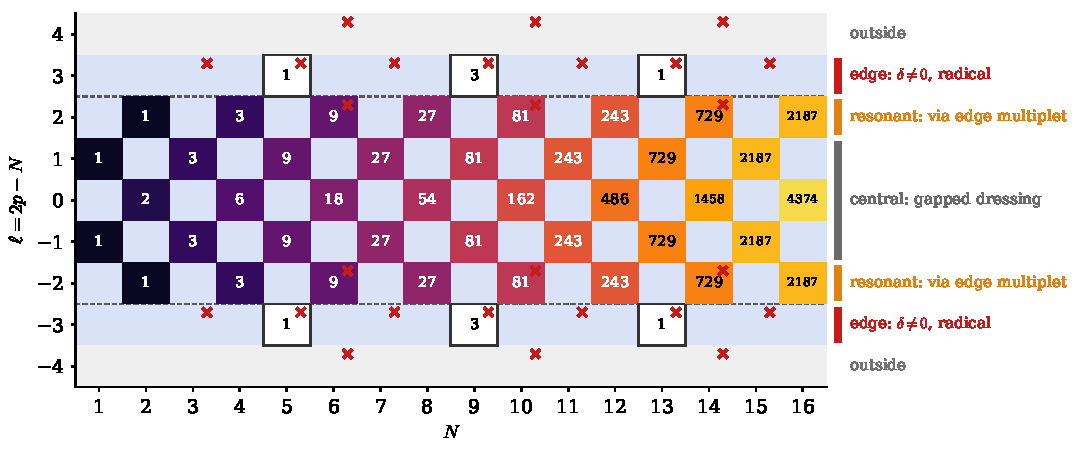
\includegraphics[width=\textwidth]{progress_2026-10-26_figs/fig_jump_map_q3.pdf}
\caption{BPS dimensions of the $q=3$ model in the $(N,\ell=2p-N)$ plane, in the conventions of CV Fig.~2. Light blue:
the fortuity window $|\ell|\le3$; dashed lines: the restricted window; white squares: exceptional states.
Right margin: the regime of the uplift \emph{into} each row $\lp$ (Sec.~\ref{sec:book}). Red crosses: sectors whose
connecting map $\delta$ is nonzero. These are the edge sectors $\lp=\pm3$ (always), $\lp=\pm2$ when $N=\Np-1\equiv1$
(mod 4) (the exchange, Sec.~\ref{sec:ranks}), and $\lp=\pm4$, where the old exceptional states are obstructed from
stepping outward. All dimensions were checked by direct computation for $\Np\le14$ in every sector, and through the
admissible-source count at $\Np=15,16$.}
\label{fig:map}
\end{figure}

\begin{figure}[p]
\centering
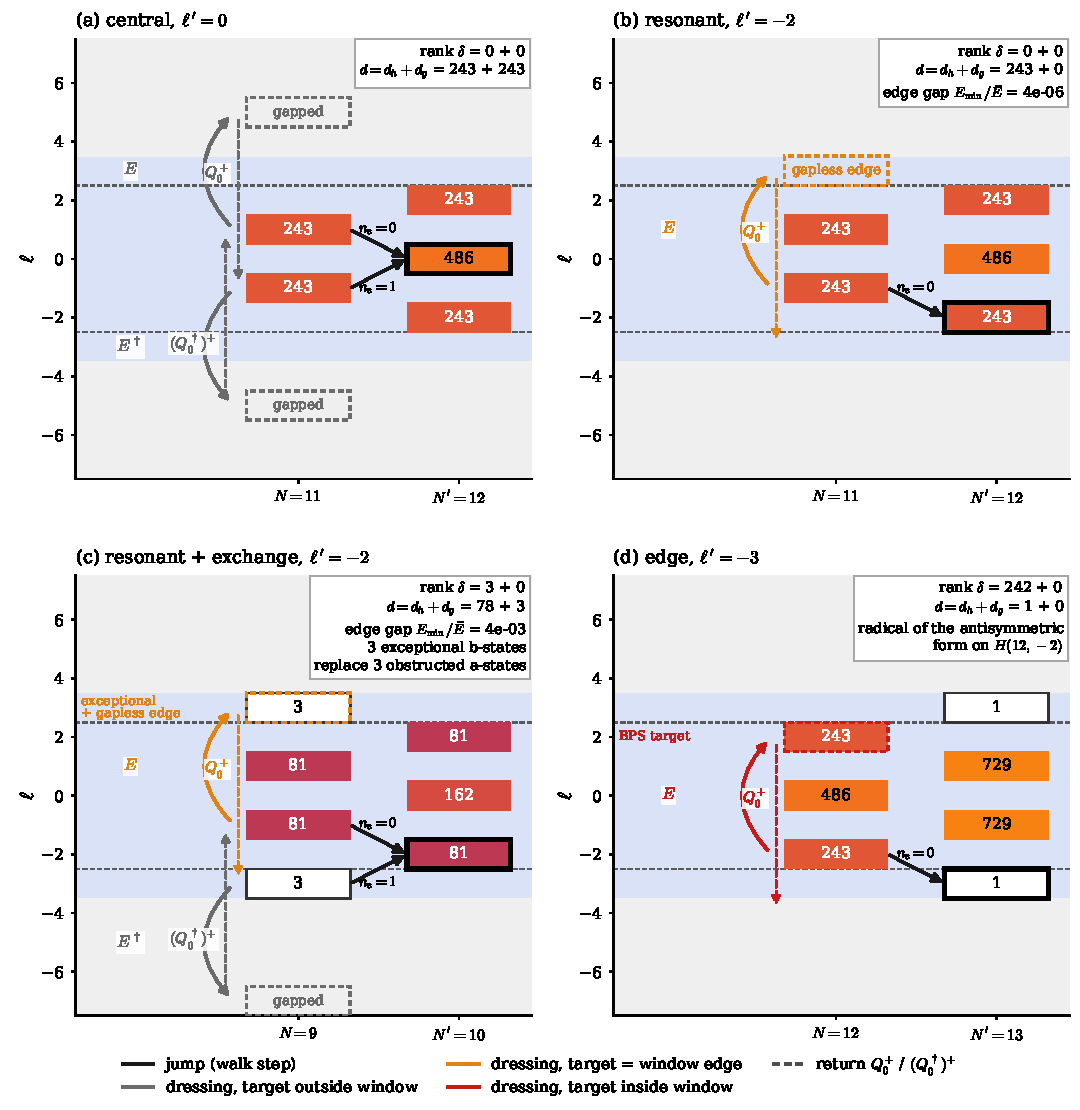
\includegraphics[width=0.97\textwidth]{progress_2026-10-26_figs/fig_jump_panels_q3.pdf}
\caption{The four kinds of uplift, each drawn as a single step $N\to\Np$ (columns), with the old and new BPS dimensions.
Black arrows: the two jumps (walk steps) from the slots at $\lp\pm1$ into the target sector (bold frame). Solid coloured
arcs: the first-order dressing by $E$ (from the $n_e=0$ slot) and $E^\dagger$ (from the $n_e=1$ slot) to their target
levels (dashed boxes). Dashed arrows: the return through $Q_0^+$ or $(Q_0^\dagger)^+$ into the other slot. Colour gives
the regime of the target: grey outside the window, orange the window edge, red inside the window. The boxes give the
measured rank of $\delta$, the admissible dimensions $d_h+d_g$, and, for resonant sectors, the gap $E_{\min}/\bar E$
of the edge multiplet (seed 9000).
(a)~Central: both loops are gapped.
(b)~Resonant: the $E$ loop passes through the gapless edge multiplet at $+3$.
(c)~Resonant with exchange ($N=9$): $\delta$ maps three ordinary classes at $-1$ onto the three exceptional states at
$+3$, and the three exceptional states at $-3$ take their place through the up step.
(d)~Edge: $E$ lands on the BPS states at $+2$, and only the radical of an antisymmetric form survives, giving the
exceptional state of $\Np=13$.}
\label{fig:panels}
\end{figure}

%=====================================================================================================================
\section{The exact uplift in every sector}\label{sec:theorem}

\begin{lemma}[\DER]\label{lem:closed}
For any $q$ odd, $E$ commutes with $Q_0$ and $E^\dagger$ with $Q_0^\dagger$, because $\eta$ has even degree $q-1$. Hence:
\begin{enumerate}\itemsep0pt
\item $E$ maps closed forms to closed forms and exact forms to exact forms ($EQ_0x=Q_0Ex$);
\item $E^\dagger$ maps coclosed forms to coclosed forms and coexact forms to coexact forms;
\item for a BPS state with $a=h+x$ ($h$ harmonic, $x$ exact) and $b=g+z$ ($z$ coexact), $\PH Ea=\PH Eh$ and
$\PH E^\dagger b=\PH E^\dagger g$.
\end{enumerate}
\end{lemma}

\begin{theorem}[\VER]\label{thm:general}
Define the connecting maps $\delta_h=\PH E\PH$ on the harmonic forms $H_X$ of the $n_e=0$ slot and
$\delta_g=\PH E^\dagger\PH$ on $H_Y$ of the $n_e=1$ slot, and the admissible sources $A_h=\ker\delta_h$,
$A_g=\ker\delta_g$. Then
\begin{equation}
B(\Np,F)=\Psi(A_h,0)\oplus\Psi(0,A_g),
\end{equation}
with $\Psi$ given by \eqref{eq:uplift}, and the sum is orthogonal. The map $(h,g)\mapsto\Psi(h,g)$ is an isomorphism, and
$\dim B=\dim\ker\delta_h+\dim\ker\delta_g$, which is CV eq.~(26).
\end{theorem}

\noindent\emph{Proof.}
\begin{itemize}\itemsep1pt
\item The BPS equations (13 October, \S2) are $Q_0a=0$, $Q_0^\dagger b=0$, $Q_0b=-\varepsilon Ea$ and
$Q_0^\dagger a=\varepsilon E^\dagger b$, independently of the sector.
\item By Lemma~\ref{lem:closed}, $Ea$ is closed. Its harmonic part is $\PH Eh$. So the third equation is solvable iff
$h\in A_h$, and similarly the fourth iff $g\in A_g$.
\item On admissible sources the solution is the anti-Hermitian system of 13 October \S5. It has a unique solution in any
sector, because $K'$ maps into exact forms and $K'K|_{\Ex}=L^\dagger L\ge0$.
\item Injectivity: $h=\PH a$ and $g=\PH b$.
\item Orthogonality: the 13 October proof uses only Lemma~\ref{lem:closed} and the Hodge decomposition. $\square$
\end{itemize}

\noindent So every closed form of 13 October holds in every sector once $B_o^F\to A_h$ and $B_o^{F-1}\to A_g$:
\begin{itemize}\itemsep1pt
\item the three operators $K_H$, $K'_H$, $L$ with $P_\Ex K'P_\Co=L^\dagger$;
\item the orthogonal splitting and the minimum-norm uplift;
\item the decoder as a generalized eigenproblem $\mathcal N v=\mu\mathcal G v$;
\item monotone self-dressing;
\item the identity $T_4=T_2-H$.
\end{itemize}

\begin{proposition}[\VER: mirror symmetry]\label{prop:mirror}
For every realization, $\operatorname{spec}\lambda(\Np,F)=1-\operatorname{spec}\lambda(\Np,\Np-F)$.
\end{proposition}
\noindent The Hodge star maps the harmonic space of the couplings $C$ at degree $F$ onto that of $\bar C$ at degree
$\Np-F$, and it exchanges $n_e\leftrightarrow1-n_e$. Complex conjugation then maps the harmonic space of $\bar C$ back to
that of $C$ without changing $n_e$. The 13 October symmetry at even $\Np$ is the self-mirror case $\lp=0$.

\paragraph{Verification \NUM.} With seeds 9000--9002, all sectors $|\lp|\le q+1$, $q=3$ at $\Np=5$--14 and $q=5$ at
$\Np=6$--14:
\begin{itemize}\itemsep1pt
\item $d_h+d_g$ equals the BPS dimension computed directly in the $\Np$-mode model, which equals the known count;
\item the uplift residual outside that space is $\le6.4\times10^{-13}$, with full rank;
\item the closed-form decoder agrees with the direct decoder to $\le2.6\times10^{-11}$;
\item the splitting overlaps are $\le1.1\times10^{-13}$;
\item Proposition~\ref{prop:mirror} holds on 39 ($q=3$) and 40 ($q=5$) sector pairs to $\le2.7\times10^{-12}$.
\end{itemize}
At $\Np=15$ the general code reproduces the exact half-filling $T_2$ of 13 October (0.5866 and 0.6013 for the two
seeds). At $\Np=16$ it gives $T_2=0.6075$ for seed 9000 at half filling, the exact value of the 13 October
pre-registered test.

%=====================================================================================================================
\section{The connecting maps}\label{sec:ranks}

\subsection{Duality and exact ranks}
\begin{lemma}[\DER]\label{lem:dual}
For harmonic $\alpha$ at level $\ell$ and $\beta$ at level $-\ell-2(q-1)$ of the $N$-mode model, define the top-form
pairing
\begin{equation}
B_\eta(\beta,\alpha)=\int\beta\wedge\eta\wedge\alpha .
\end{equation}
Then:
\begin{enumerate}\itemsep0pt
\item $\beta\mapsto\overline{\star\beta}$ is an antilinear bijection between harmonic spaces at levels $\pm\ell$, so the
matrix of $\delta$ on $H(N,\ell)$ is that of $B_\eta$;
\item $\operatorname{rank}\delta|_{H(\ell)}=\operatorname{rank}\delta|_{H(-\ell-2(q-1))}$;
\item on the self-paired level $\ell=1-q$, with $k=(N-q+1)/2$, $B_\eta(\alpha,\beta)=(-1)^kB_\eta(\beta,\alpha)$.
\end{enumerate}
\end{lemma}
\noindent Part~3 holds because $\eta$ has even degree, so moving $\beta$ (degree $k$) to the front costs $(-1)^{k^2}=(-1)^k$.

\begin{proposition}[exact ranks, $q=3$; \DER\ given the window premise, \NUM\ verified]\label{prop:ranks}
Let $e(N)$ be the number of exceptional states of the $N$-mode model per edge. For the uplift into level $\lp$:

\begin{center}\small
\begin{tabular}{ccccc}
\toprule
$\lp$ & $\delta_h$: source $\to$ target & rank $\delta_h$ & $A_h$ & $A_g$\\
\midrule
$0,\pm1$ & target outside window & 0 & $H_X$ & $H_Y$\\
$-2$ & $H(N,-1)\to H(N,+3)$ & $e(N)$, onto & codim $e(N)$ & $H(N,-3)$ ($e(N)$ exceptional)\\
$-3$ & $H(N,-2)\to H(N,+2)$ & $3^{N/2-1}-e(\Np)$ & radical of $B_\eta$ & 0\\
$-4$ & $H(N,-3)\to H(N,+1)$ & $e(N)$, injective & 0 & 0\\
\bottomrule
\end{tabular}
\end{center}
\noindent Positive $\lp$ is the mirror, with $\delta_g$.
\end{proposition}
\noindent\emph{Derivation.}
\begin{itemize}\itemsep1pt
\item Row $\lp=-4$ restates the window premise at $\Np$: there are no BPS states at $|\lp|>q$ (KW eq.~6.15; CV eq.~12).
\item Lemma~\ref{lem:dual} pairs $H(N,-3)$ with $H(N,-1)$, so row $\lp=-2$ has the same rank as row $\lp=-4$. This is
the surjectivity.
\item Row $\lp=-3$ is the self-paired form.
\end{itemize}
\NUM\ All 142 $q=3$ sector records ($\Np\le16$) and all 114 $q=5$ records agree with these ranks. For $q=5$ the same
table holds with levels $\pm4,\pm5,\pm6$ in place of $\pm2,\pm3,\pm4$.

\paragraph{The exchange \DER.} At $\lp=-2$ with $N\equiv1$ (mod 4) there are two competing effects.
\begin{itemize}\itemsep1pt
\item $e(N)$ ordinary classes of $H(N,-1)$ are obstructed: their dressing would have to land on the exceptional states
at $+3$.
\item The $e(N)$ exceptional states at $-3$ cannot step down (row $\lp=-4$). They step up instead.
\end{itemize}
The dimension $3^{(N-1)/2}$ is unchanged, as CV's strip-walk count requires. But the uplift is not a walk-by-walk
bijection: an exceptional class is created at the edge (next subsection), and leaves by an up step that displaces one
ordinary class (Fig.~\ref{fig:panels}c).

\subsection{Exceptional states are a radical}
At the edge $\lp=-q$ the $n_e=1$ slot is empty, so $B(\Np,-q)=\ker\delta_h$ on $H(N,1-q)$. This is the radical of
$B_\eta$ on the self-paired level. An antisymmetric form on an odd-dimensional space always has a nonzero radical, which
gives the following.

\begin{theorem}[\DER]\label{thm:radical}
The exceptional BPS states of the $\Np$-mode model at level $-q$ form the radical of $B_\eta$ on $H(\Np-1,1-q)$. If
$k=(\Np-q)/2$ is odd and $\dim H(\Np-1,1-q)$ is odd, there is at least one.
\end{theorem}

\noindent Remarks on Theorem~\ref{thm:radical}.
\begin{itemize}\itemsep1pt
\item For $q=3$, $\dim H(N,-2)=3^{N/2-1}$ is odd, so the condition is $\Np\equiv1$ (mod 4). This is the uplift form of
KW's Kramers argument (KW \S6.2) and of CV eq.~(15).
\item The parity is the same as in CV's version. CV's antisymmetric $M$ on $\Lambda^a(\Np)$ gives
$\dim\mathrm{harm}\equiv\tilde D_a(\Np)$. Our condition involves
$S_{\Np-1}(1-q)=\tilde D_a(\Np-1)-\tilde D_{a-1}(\Np-1)$, while $\tilde D_a(\Np)=\tilde D_a(\Np-1)+\tilde D_{a-1}(\Np-1)$,
in the notation of CV App.~A.
\item \NUM\ The forms are exactly (anti)symmetric: $|B^T-(-1)^kB|/|B|\le4.3\times10^{-15}$.
\begin{itemize}\itemsep0pt
\item $q=3$: radicals $1,3,1$ at $N=4,8,12$, and 0 at $N=6,10,14$.
\item $q=5$: radical 1 at $N=6,10$. At $N=14$ the form is antisymmetric but $\dim=1000$ is even, and the radical
vanishes, matching KW's ``no exceptional modes at $N_c=15$''.
\item The singular values of the antisymmetric forms come in equal pairs.
\end{itemize}
\end{itemize}

\paragraph{Beyond KW's range \DER.} Theorem~\ref{thm:radical} forces exceptional states, for $\Np\le45$, at:
\begin{center}\small
\begin{tabular}{ll}
\toprule
$q$ & $\Np$ with forced exceptional states\\
\midrule
3 & all $\Np\equiv1$ (mod 4)\\
5 & 7, 11, 19, 23, 31, 35, 43\\
7 & 9, 21, 25, 29, 37\\
9 & 11, 15, 23, 39, 43\\
\bottomrule
\end{tabular}
\end{center}
KW tested $\hat q=5$ only up to $N_c=17$, finding edge modes only at 7 and 11. For $\Np=19$ the statement is rigorous for
generic couplings:
\begin{itemize}\itemsep1pt
\item CV's $M$ on $\Lambda^7(19)$ is antisymmetric on the even dimension 50388;
\item $Q$ is injective on $\Lambda^2(19)$: rank 171 for two realizations, with $\sigma_{\min}/\sigma_{\max}=0.89$, which
implies the same for generic couplings;
\item so the exact 7-forms have dimension 171, and $\dim H^7\equiv0-171\equiv1$ (mod 2).
\end{itemize}
Figure~\ref{fig:q5} shows the $q=5$ plane with its regimes.

\paragraph{Not explained.} At $\Np=9$ ($q=3$) the radical has dimension 3, not 1: this is KW's excess. The radical
\emph{subspace} moves with $\eta$ (principal-angle cosines between different $\eta$ are 0.05--0.49), but its dimension is
3 for every $\eta$ we tried. We have no structural reason for this.

\begin{figure}[t]
\centering
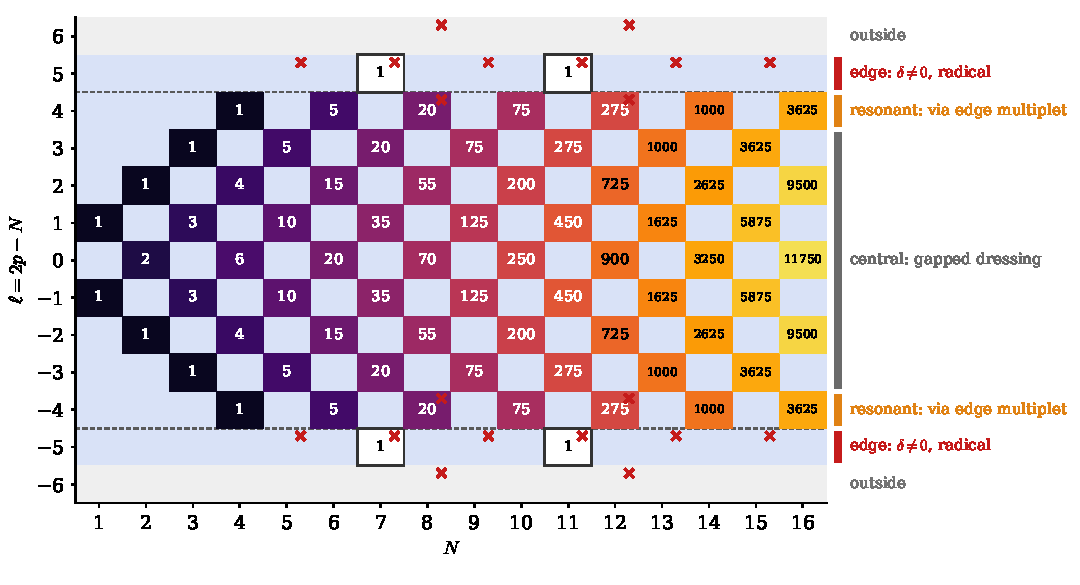
\includegraphics[width=\textwidth]{progress_2026-10-26_figs/fig_jump_map_q5.pdf}
\caption{As Fig.~\ref{fig:map} for $q=5$, to be compared with CV Fig.~3. Every entry up to $N=13$ agrees with CV. The
resonant rows are $\lp=\pm4$ and the edge rows $\lp=\pm5$. Exceptional states appear at $N=7,11$ (KW). The parity
criterion puts the next ones at $N=19$.}
\label{fig:q5}
\end{figure}

%=====================================================================================================================
\section{Dressing: gapped, resonant, obstructed}\label{sec:dressing}

\subsection{The two-point function in the three regimes}
By the 13 October report, the first-order dressing cost of an admissible source is a BPS-projected, Euclidean-time-integrated
two-point function of $E$:
\begin{equation}
\sigma^2\in\operatorname{spec}\,P E^\dagger H_0^{+}EP=\operatorname{spec}\int_0^\infty d\tau\,P E^\dagger e^{-\tau H_0}EP\qquad(\text{on }\ker\delta).
\end{equation}
For a \emph{non-admissible} source the integrand tends to $\|\delta h\|^2$ at late times, and the integral grows
linearly. \textbf{The obstruction is the late-time plateau of the two-point function}, which in chord language is the
BPS$\to$BPS weight: the point mass of the 14 October Al-Salam--Chihara measure, equal to BLY eq.~(4.14)~\cite{BLY}.

In the chord limit, the 14 October closed form gives \CHORD
\begin{gather}
G(\tau)=\int_0^\pi\! d\phi\,f(\phi)\,e^{-\tau\kappa\Lambda(\phi)},\qquad
\Lambda(\phi)=2q^{-1/2}\big[\cosh\lambda(s_{\rm in}-\tfrac12)-\cos\phi\big],\\
f(\phi)=\frac{(ab;q^2)_\infty(q^2,e^{\pm2i\phi};q^2)_\infty}{2\pi(ae^{\pm i\phi},be^{\pm i\phi};q^2)_\infty},
\end{gather}
with $a=q^{s_{\rm in}-1/2}$ and $b=q^{1/2+\delta-s_{\rm out}}$. Its late-time behaviour depends on the regime.
\begin{itemize}\itemsep1pt
\item $s_{\rm in}>\tfrac12$ (gapped): $a<1$, so $f\propto\phi^2$ near $\phi=0$, while $\Lambda\simeq\Lambda_{\min}+q^{-1/2}\phi^2$.
Hence $G(\tau)\sim\tau^{-3/2}e^{-\kappa\Lambda_{\min}\tau}$.
\item $s_{\rm in}=\tfrac12$ (resonant): $a=1$. The zero of $(e^{\pm2i\phi};q^2)$ is cancelled by that of
$(e^{\pm i\phi};q^2)$, so $f(0)=2(q^2;q^2)_\infty/[\pi(b;q^2)_\infty]$ is finite, while $\Lambda\simeq q^{-1/2}\phi^2$.
Hence
\begin{equation}
G(\tau)\simeq\frac{f(0)}2\sqrt{\frac{\pi q^{1/2}}{\kappa\tau}}\ \propto\ \tau^{-1/2},
\end{equation}
and $\int G\,d\tau$ diverges. Consistently, the 14 October closed form
$\propto{}_2\phi_1(q^2,q^2;q^{2+2\delta};q^2,q^{2s_{\rm in}-1})$ has terms that tend to a constant as $s_{\rm in}\to\tfrac12^+$,
which gives a pole $\propto1/\lambda(2s_{\rm in}-1)$.
\item $s_{\rm in}<\tfrac12$ (obstructed): a point mass at zero energy, i.e.\ the plateau.
\end{itemize}

\subsection{The resonant tail}
The 14 October report showed that, for uncrossed chord diagrams, the first-order dressing operator is free compound Poisson.
Its jump law is $g(\phi)\propto A(\phi)/\Lambda(\phi)$ under the B-family density, at rate $r$ = (inner modes)/(sources).
At $s_{\rm in}=\tfrac12$ the jumps are unbounded: $g\simeq G_0/\phi^2$ as $\phi\to0$, while the density tends to a finite
$\rho_0$. A single large jump produces a single large eigenvalue, so \CHORD
\begin{equation}\label{eq:tail}
P(\sigma^2>K)\simeq r\,w(g>K)\simeq r\rho_0\sqrt{G_0}\;K^{-1/2}.
\end{equation}
The mean is therefore infinite in the chord limit; at finite $N$ the smallest inner energy cuts it off. The amplitude
is parameter-free. From the 14 October chord functions at $(s_{\rm out},s_{\rm in})=(-\tfrac16,\tfrac12)$:
$P\sqrt K=0.50$, $0.51$, $0.52$ at $\Np=12$, $14$, $16$.

\subsection{Finite \texorpdfstring{$N$}{N}}
\begin{itemize}\itemsep1pt
\item \DER\ \emph{Which multiplet.} By the bookkeeping \eqref{eq:path}, the resonant family dresses through
coexact$(-q)\leftrightarrow$exact$(+q)$, which is exactly KW's GOE/GSE multiplet.
\INTERP\ It is also the only multiplet in which $Q_0$ maps between ambient spaces of equal dimension,
$\binom{N}{(N-q)/2}=\binom N{(N+q)/2}$. That would explain a ``square'' hard edge at zero.
\item \NUM\ \emph{Its gap.} The seed means are $E_{\min}/\bar E=2.5\times10^{-1}$, $2.1\times10^{-2}$, $2.9\times10^{-3}$,
$5.9\times10^{-6}$, $1.6\times10^{-6}$ at $N=5,7,9,11,13$, and $8.0\times10^{-8}$ and $1.5\times10^{-10}$ (two seeds) at $N=15$ (Fig.~\ref{fig:res}a). Gapped
families stay at $0.02$--$0.6$. In units of the multiplet dimension $n$ ($=4,21,80,319,1208,4551$),
$n^2E_{\min}/\bar E$ stays at $0.003$--$24$ per seed ($0.15$--$13$ for $q=5$). This is the hard-edge scaling of a square
random matrix \INTERP: $E_{\min}$ is exponentially small in $N$ because $n$ is exponentially large. The smallest values
($0.003$ and $0.06$) occur in the GOE multiplets ($N\equiv3$ mod 4), as the softer $\beta=1$ hard edge
($P(n\sigma_{\min}<x)\propto x$) would suggest; the Kramers (GSE) multiplets never go below $1.1$. With 2--3 seeds per $N$
this is suggestive only.
\item \NUM\ \emph{Dominance of the bottom.} The lowest 1\% of inner modes carries 90\%, 96\% and 99\% of the
first-order dressing trace at $N=11,13,15$, against $\le14\%$ in gapped families.
\item \NUM\ \emph{Dressing costs.} The seed-mean is $1.3$, $4.1$, $7.0$, $1244$, $851$, $1579$ and $6.6\times10^5$ (two seeds; the latter from one mode with $E/\bar E=1.5\times10^{-10}$, and 613 and 688 without the top state) at
$\Np=6,8,10,12,14,16$; the median $0.14$--$0.74$; the maximum $1.45\times10^{9}$. Central sectors have mean $\le0.42$ and
maximum $\le5.2$. Single modes dominate the mean, which therefore fluctuates strongly from seed to seed, as a
$K^{-1/2}$ tail requires.
\item \NUM\ \emph{The tail} (Fig.~\ref{fig:res}b). $P(\sigma^2>K)\propto K^{-\alpha}$ over four decades.
\begin{itemize}\itemsep0pt
\item The Hill estimate of $\alpha$ (for $K>100$; $h$ family at $\lp=-2$, all seeds) is $0.43\pm0.06$ at $\Np=12$
($n=48$), $0.48\pm0.04$ at $\Np=14$ ($n=144$), and $0.48\pm0.03$ ($n=259$) at $\Np=16$.
\item The chord value \eqref{eq:tail} is $\alpha=\tfrac12$. The measured amplitude at $K=100$ is $P\sqrt K=0.66$,
$0.66$, 0.59 at $\Np=12,14,16$, against the chord $0.50$, $0.51$, $0.52$.
\item The ratio of data to chord amplitude falls with $\Np$ ($1.32$, $1.29$, 1.13), toward the chord law.
\end{itemize}
\item \NUM\ \emph{$q=5$.} The same happens at $|\lp|=4$ and nowhere else: gap $8.1\times10^{-5}$ ($N=11$) and
$7.5\times10^{-7}$ ($N=13$); mean dressing 98 and 1070.
\end{itemize}

\begin{figure}[t]
\centering
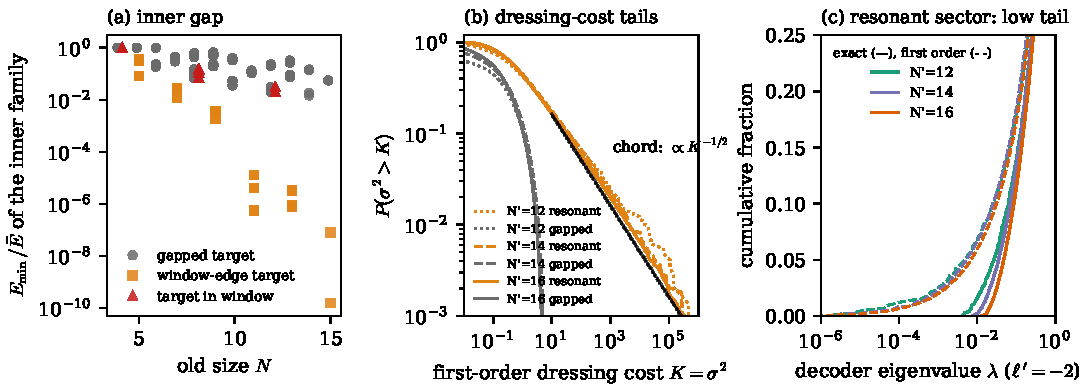
\includegraphics[width=\textwidth]{progress_2026-10-26_figs/fig_resonance.pdf}
\caption{The window-edge resonance.
(a)~Gap $E_{\min}/\bar E$ of the inner family (the old energies through which each dressing family passes) against the
old size $N$, coloured by regime. The window-edge multiplet (orange) closes to $\sim10^{-6}$; gapped families do not.
(b)~Fraction of sources with first-order dressing cost above $K$. Orange: resonant families ($\lp=\pm2$); grey: central
families. Black: the parameter-free chord tail $r\,w(g>K)$ of Eq.~\eqref{eq:tail} at the same $\Np$, $\propto K^{-1/2}$.
(c)~Cumulative distribution of the lowest decoder eigenvalues in the resonant sector $\lp=-2$: first order (dashed)
against exact (solid). First order places resonant states down to $\lambda\sim10^{-7}$--$10^{-9}$ (clipped at
$10^{-7}$); the exact decoder stops near $10^{-2}$. All panels pool the available seeds (3; 2 at $\Np=16$).}
\label{fig:res}
\end{figure}

\subsection{What the exact uplift does with the resonance}
Write $Q_0=\sum_js_j|u_j\rangle\langle v_j|$ on the inner multiplet, and $e=U^\dagger EV_h$. The self-dressed metric
block of 13 October is then exactly \DER
\begin{equation}
K_H^\dagger(1+R)^{-1}K_H=e^\dagger(S^2+W)^{-1}e,\qquad W=U^\dagger EP_\Ex E^\dagger U=SRS .
\end{equation}
This is the first-order dressing with the propagator of $H_0+EP_\Ex E^\dagger$ in place of $H_0^{-1}$: a Dyson resummation
whose self-energy is $EP_\Ex E^\dagger$ (verified to $4\times10^{-15}$).

But $[E,Q_0]=0$ forces the self-energy to be ``soft'': $W_{jj}=s_j^2R_{jj}$, with $R_{jj}$ bounded (measured
$0.06$--$0.14$ on the lowest modes). It vanishes on the near-zero modes. \textbf{So the resonance survives in the exact
minimum-norm dressing cost} \NUM: the mean is 1190 against 1244 at first order ($\Np=12$), 787 against 851 ($\Np=14$),
and 1454 against 1579 and $6.1\times10^5$ against $6.6\times10^5$ (two seeds) ($\Np=16$).

\textbf{The decoder angles do not resonate.} For a state whose cloud dominates, the exact $h$ block gives \DER
\begin{equation}
\lambda\to1-\frac{\ip{\hat k}{(1+R)^{-2}\hat k}}{\ip{\hat k}{(1+R)^{-1}\hat k}},
\end{equation}
which is set by the bounded operator $R$, not by $\sigma$. \NUM\ First order puts 2.0--2.5\% of resonant-sector states
within $10^{-3}$ of the wall, its lowest eigenvalue being $10^{-7}$--$10^{-5}$. The exact decoder has none there, and at
$\Np=16$ none within $10^{-2}$. Its floor rises with $\Np$: the lowest eigenvalue is $(4.5$--$6.5)\times10^{-3}$ at
$\Np=12$, $(8$--$10)\times10^{-3}$ at $\Np=14$, and $(1.4$--$1.5)\times10^{-2}$ (first order: $5\times10^{-7}$, $7\times10^{-10}$) at $\Np=16$ (Fig.~\ref{fig:res}c). The 13 October per-mode mean field, which replaces $R$ by its diagonal, fails here: its $T_2$
is low by $0.04$--$0.05$. The spread of $R$ along the resonant direction matters.

\paragraph{Reading \INTERP.}
\begin{itemize}\itemsep1pt
\item In resonant sectors, a few BPS states of $\Np$ are made mostly of the near-zero modes of the old edge multiplet,
i.e.\ of states that are almost BPS at the window edge $s=\pm\tfrac12$.
\item Their harmonic seed carries a vanishing fraction of the norm, $\|h\|^2/\|\Psi\|^2\sim1/\kappa$. This is CV's
metric fragility in its strongest form, localized at $|\lp|=q-1$.
\item In chord language, these sectors are where the uplift's matter chord ends on the gapless $Q=\tfrac12$ supermultiplet
of the super-Schwarzian. This is HITZ App.~A~\cite{HITZ}, as already used for two flavors in the 25 October
report~\cite{prog1025}, whose resonances at $s'=\pm\tfrac15$ are the analogue.
\end{itemize}

%=====================================================================================================================
\section{The decoder across the window}\label{sec:decoder}

\begin{table}[h]
\centering\small
\resizebox{\textwidth}{!}{%
\begin{tabular}{rrrcccc}
\toprule
$\Np$ & $\lp$ & $d$ ($h$+$g$) & $T_2$: first $\to$ self $\to$ exact & $H$: first / exact & $T_4-(T_2-H_{\rm first})$ & walls$(10^{-3})$: first / exact\\
\midrule
12 & 0  & 486 (243+243) & 0.631 $\to$ 0.670 $\to$ 0.685 & 0.085 / 0.090 & $-0.0045$ & 0.329 / 0.329\\
12 & $-2$ & 243 (243+0) & 0.515 $\to$ 0.497 $\to$ 0.497 & 0.125 / 0.132 & $-0.0069$ & 0.025 / 0.000\\
13 & $-1$ & 729 (486+243) & 0.563 $\to$ 0.604 $\to$ 0.616 & 0.111 / 0.109 & $+0.0026$ & 0.112 / 0.123\\
13 & $-3$ & 1 (1+0) & $\lambda=0.65,\,0.58,\,0.65$ (one exceptional state) & -- & -- & --\\
14 & 0 & 1458 (729+729) & 0.566 $\to$ 0.619 $\to$ 0.636 & 0.105 / 0.108 & $-0.0034$ & 0.116 / 0.128\\
14 & $-2$ & 729 (728+1) & 0.477 $\to$ 0.455 $\to$ 0.455 & 0.133 / 0.142 & $-0.0092$ & 0.023 / 0.000\\
16 & 0 & 4374 (2187+2187) & 0.539 $\to$ 0.595 $\to$ 0.608 (1 seed) & 0.122 / 0.125 & $-0.0030$ & 0.011 / 0.021\\
16 & $-2$ & 2187 (2187+0) & 0.452 $\to$ 0.427 $\to$ 0.427 & 0.138 / 0.148 & $-0.0106$ & 0.020 / 0.000\\
\bottomrule
\end{tabular}}
\caption{Decoder statistics by sector (3 seeds; at $\Np=16$, 2 seeds). ``Self'' is the exact uplift without the $h$--$g$
mixing. Walls: the fraction with $\min(\lambda,1-\lambda)<10^{-3}$. In central sectors these are the exact atoms of
13 October; in resonant sectors they are first-order artifacts.}
\label{tab:decoder}
\end{table}

\begin{itemize}\itemsep1pt
\item \NUM\ \emph{The $T_4$ prediction.} $T_4=T_2-H$ is exact. The first-order prediction $T_4\simeq T_2-H_{\rm first}$
of 13 October holds to $\le0.009$ in every extensive sector at $\Np=9$--14, and to $\le0.011$ at $\Np=16$
(Fig.~\ref{fig:dec}b, Table~\ref{tab:decoder}). It is not uniform across the window, though.
\begin{itemize}\itemsep0pt
\item In resonant sectors the error grows steadily: $-0.0069$, $-0.0092$, $-0.0106$ at $\Np=12,14,16$.
\item In central sectors it shrinks: $-0.0045$, $-0.0034$, $-0.0030$.
\item The first-order spectrum of resonant sectors is visibly wrong at the bottom, so this degradation is expected.
\end{itemize}
\item \NUM\ \emph{Self-dressing lowers $T_2$ in resonant sectors.} Cloud-dominated states move away from the $\lambda=0$
wall, so $y=\mu^2$ drops from about 1. In central sectors self-dressing raises $T_2$.
\item \DER+\NUM\ \emph{Atoms.} The 13 October count generalizes: forced atoms $=\max(0,\dim A-\dim(\text{target family}))$.
At $\lp=-2$ the target family is the edge multiplet. At $\Np=8$ this forces $27-21=6$ atoms, observed in every seed;
none are forced from $\Np=10$ on.
\item \NUM\ \emph{Exceptional states.} At $\lp=-q$ they are $h$-type, carrying 58--76\% of their weight in $n_e=0$ at
$\Np=5,13$ (0.27--0.79 at $\Np=9$).
\item \NUM\ \emph{The exceptional states that uplift at $\lp=-2$} (the exchange) have gapped dressing, with
$\lambda_1=0.02$--$0.13$. At $\Np=10$ they remain separate states near $\lambda=0.003$--$0.02$. At $\Np=14$ the single
one dissolves into the resonant $h$ block: no exact eigenvector has more than 5--9\% weight on it.
\end{itemize}

\begin{figure}[t]
\centering
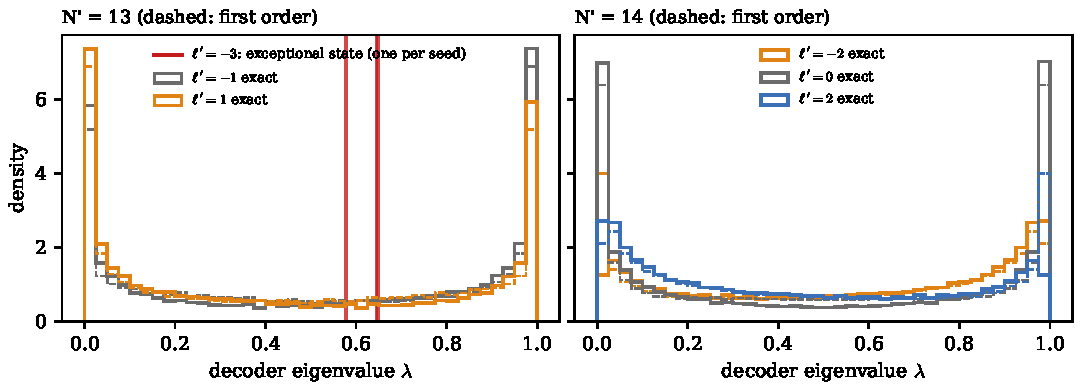
\includegraphics[width=0.66\textwidth]{progress_2026-10-26_figs/fig_decoder_sectors.pdf}\hfill
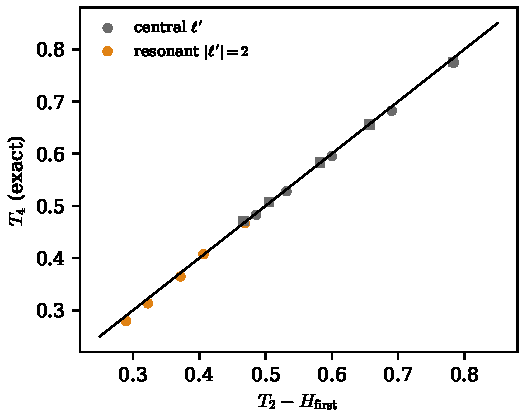
\includegraphics[width=0.32\textwidth]{progress_2026-10-26_figs/fig_T4_sectors.pdf}
\caption{(a)~Decoder densities at $\Np=13$ (left) and $\Np=14$ (middle) by sector; solid exact, dashed first order.
Mirror sectors are reflections of each other. At $\Np=13$ the vertical lines are the single exceptional state at
$\lp=-3$ (one per seed). (b)~Right: exact $T_4$ against the first-order prediction $T_2-H_{\rm first}$. Circles are
even $\Np$, squares odd $\Np$, for all extensive sectors with $\Np=6$--16; the line is $T_4=T_2-H_{\rm first}$.}
\label{fig:dec}
\end{figure}

%=====================================================================================================================
\section{Discussion}\label{sec:discussion}

\subsection{What changes off half filling}
Three things change, and each has a precise location on the jump map.
\begin{enumerate}\itemsep1pt
\item \emph{Cohomology} (CV's $\delta$) acts only at the edge rows $|\lp|=q$, at the exchange rows $|\lp|=q-1$ when the
old model has exceptional states, and at $|\lp|=q+1$.
\item \emph{Metric resonance} acts only at $|\lp|=q-1$.
\item Everywhere else the 13 October picture holds unchanged.
\end{enumerate}
Exceptional states acquire a life cycle. They are born as a radical at the edge, and leave by displacing one ordinary
class one step inside.

\subsection{What is established, and how firmly}
\begin{itemize}\itemsep1pt
\item \emph{Exact.}
\begin{itemize}\itemsep0pt
\item Theorem~\ref{thm:general} and its corollaries, and Proposition~\ref{prop:mirror};
\item the duality and (anti)symmetry of $B_\eta$, Theorem~\ref{thm:radical}, and the parity criterion;
\item $q=5$, $\Np=19$, given one rank computation;
\item the Dyson identity with $W=SRS$, and the cloud-dominated limit of $\lambda$.
\end{itemize}
\item \emph{Exact given the window premise} (KW 6.15, CV Conj.~A.1, both verified to $N\le17$): the rank table and the
exchange.
\item \emph{Derived from the chord rules:} the three late-time behaviours, and the $K^{-1/2}$ tail with its amplitude.
\item \emph{Numerical:}
\begin{itemize}\itemsep0pt
\item the machine-precision verification;
\item the hard edge of the edge multiplet;
\item the tail exponent and amplitude;
\item the absence of a wall pile-up in the exact decoder;
\item $T_4\simeq T_2-H_{\rm first}$ in every sector, though slowly degrading in resonant sectors.
\end{itemize}
\item \emph{Heuristic or interpretive:} the ``square'' explanation of the hard edge, and the reading of cloud-dominated
states as BPS states assembled from the old edge continuum.
\end{itemize}

\subsection{Limitations}
\begin{itemize}\itemsep1pt
\item Sizes: $\Np\le16$ with dense linear algebra, and 1--3 seeds per sector (2 for the $\Np=16$ resonant sector,
1 for the $\Np=16$ central sector).
\item The resonant tail is measured over at most four decades, with $\lesssim260$ events above $K=100$. The amplitude
agrees to 13--32\%, improving with $\Np$, and the effective exponent is still drifting. A single near-zero mode can
dominate the mean dressing cost of a realization (seed 9001 at $\Np=16$).
\item The exponentially small edge gap makes numerical rank decisions delicate. At $\Np=16$ one record (seed 9001)
first failed the dimension check: a coexact edge mode with $\sigma/\sigma_{\max}\sim10^{-5}$ fell below a Gram-eigenvalue
threshold. Ranks are now decided by singular values, consistently with the pseudo-inverse, and the record was rerun.
Sizes beyond $\Np\approx18$ will need rank decisions informed by the known dimensions, or higher precision.
\item The chord prediction \eqref{eq:tail} keeps only uncrossed diagrams and the rank-one large-jump approximation. The
14 October report measured crossed diagrams at $\le0.5\%$ of the third moment in central sectors. This has not been
checked for heavy tails.
\end{itemize}

\subsection{Open problems}
\begin{itemize}\itemsep1pt
\item The rank deficit at $\Np=9$ (radical 3 instead of 1).
\item The large-$N$ laws of $E_{\min}$ and of the tail amplitude. Sparse or partial methods could reach $\Np=18$, since
only the lowest edge modes matter.
\item A closed form for the exact resonant decoder edge, $\lambda_{\min}\sim10^{-2}$: the spectral measure of $R$ along the
resonant modes.
\item The two-flavor counterpart of the radical criterion and of the exchange.
\item Whether the cloud-dominated states have a direct gravitational description, as BPS states of $\Np$ built from the
gapless edge continuum of $N$.
\end{itemize}

%=====================================================================================================================
\appendix
\section{Verification summary}\label{app:verify}
\begin{center}\small
\begin{tabular}{p{0.52\textwidth}p{0.4\textwidth}}
\toprule
check & result\\
\midrule
KW App.~B rows from our rank computations ($N=5,9,12,13$) & exact match\\
dimensions: admissible = direct = strip walks + exceptional ($q=3$: $\Np\le14$ direct, 15--16 admissible; $q=5$: $\le14$) & all sectors, all seeds\\
connecting-map ranks vs Proposition~\ref{prop:ranks} & 142 ($q=3$) + 114 ($q=5$) records, all equal\\
uplift residual / rank & $\le6.4\times10^{-13}$ / full\\
closed-form vs direct decoder & $\le2.6\times10^{-11}$\\
orthogonal splitting & $\le1.1\times10^{-13}$\\
mirror symmetry (Prop.~\ref{prop:mirror}) & $\le2.7\times10^{-12}$ (79 pairs)\\
(anti)symmetry of $B_\eta$; radicals & $\le4.3\times10^{-15}$; $1,3,1$ / $1,1,0$ as predicted\\
$Q|_{\Lambda^2(19)}$ injective ($q=5$) & rank 171, $\sigma_{\min}/\sigma_{\max}=0.89$\\
Dyson identity $W=SRS$ & $\le4\times10^{-15}$\\
monotone self-dressing (single-family sectors) & 50 sectors; violations $\le3\times10^{-11}$ (round-off)\\
$T_2$ at half filling vs 13 October & $\Np=15$: 0.5866, 0.6013 (D6: 0.587, 0.601); $\Np=16$: 0.6075 (= D6)\\
unit tests & \url{test_uplift_window.py} (9), \url{test_uplift.py} (6), \url{test_chord_dressing.py} (8), all in \url{tests/}\\
\bottomrule
\end{tabular}
\end{center}

\section{Numerical methods and reproducibility}\label{app:repro}

\paragraph{Code.} All code is at commit \texttt{1ad5bb9}.
\begin{itemize}\itemsep1pt
\item \texttt{src/uplift.py}: \texttt{OldModel(F=)}, \texttt{harmonic\_basis}, \texttt{uplift\_bookkeeping},
\texttt{connecting\_form}, \texttt{OldModel.dyson}. Half-filling behaviour is unchanged, and the existing tests pass.
\item \texttt{src/chord\_dressing.py}: \texttt{chord\_sectors(F=)}.
\item Scripts: \url{scripts/run_uplift_window.py} (tasks \texttt{sectors}, \texttt{forms}),
\url{scripts/analyze_uplift_window.py} and \url{scripts/plot_uplift_window_map.py}.
\end{itemize}

\paragraph{Couplings.} $c=$\texttt{random\_couplings(default\_rng(seed), C(N',q))}, shared by all sectors of one
$(\Np,\text{seed})$. At $q=3$ and half filling these are the realizations of the 13 October data (seeds 9000, 9001).

\paragraph{Runs.} All under \url{scripts/memwatch.py}, with outputs in
\url{results/data/uplift_window_2026-10-26/}:
\begin{itemize}\itemsep1pt
\item $q=3$, $\Np=5$--14, seeds 9000--9002: peak 0.83\,GB, 919\,s;
\item $q=5$, $\Np=6$--14, seeds 9000--9001: peak 1.51\,GB, 1048\,s;
\item connecting forms: peak 0.50\,GB;
\item $q=3$, $\Np=15,16$, $\lp\le0$, seeds 9000--9001: the run that also did $\Np=15$ peaked at 7.82\,GB (3653\,s), and was stopped by hand after its last needed record; the seed-9001 rerun peaked at 5.42\,GB (1261\,s).
\end{itemize}
Two first launches crashed before writing any record (an empty-family bug, since fixed). One $\Np=16$ record was
rerun after the rank-decision fix described in Sec.~\ref{sec:discussion}. Both incidents are recorded in
\url{research/notes/uplift_window_2026-10-26.md}.

\paragraph{Analysis.} \texttt{analyze\_uplift\_window.py} writes \texttt{summary.json} and \texttt{chord\_tail.json}.
The chord tail uses the 14 October functions at $(s_{\rm out},s_{\rm in},\delta)=(-\tfrac16,\tfrac12,\tfrac23)$ with
4000 Gauss--Legendre nodes.

\begin{thebibliography}{99}\small
\bibitem{CV} J.~Chryssanthacopoulos and D.~Vegh, \emph{Fortuity and fragility in supersymmetric SYK}, arXiv:2608.12160 (2026).
\bibitem{KW} T.~Kanazawa and T.~Wettig, \emph{Complete random matrix classification of SYK models with $\mathcal N=0$, 1 and 2 supersymmetry}, JHEP 09 (2017) 050, arXiv:1706.03044.
\bibitem{FGMS} W.~Fu, D.~Gaiotto, J.~Maldacena and S.~Sachdev, \emph{Supersymmetric Sachdev-Ye-Kitaev models}, Phys.\ Rev.\ D \textbf{95} (2017) 026009, arXiv:1610.08917.
\bibitem{CCSY} C.-M.~Chang, Y.~Chen, B.~S.~Sia and Z.~Yang, \emph{Fortuity in SYK models}, arXiv:2412.06902.
\bibitem{BBNR} M.~Berkooz, N.~Brukner, V.~Narovlansky and A.~Raz, \emph{The double scaled limit of super-symmetric SYK models}, JHEP 12 (2020) 110, arXiv:2003.04405.
\bibitem{BLY} J.~Boruch, H.~W.~Lin and C.~Yan, \emph{Exploring supersymmetric wormholes in $\mathcal N=2$ SYK with chords}, arXiv:2308.16283.
\bibitem{TW} G.~J.~Turiaci and E.~Witten, \emph{$\mathcal N=2$ JT supergravity and matrix models}, arXiv:2305.19438 (2023).
\bibitem{HITZ} M.~Heydeman, L.~V.~Iliesiu, G.~J.~Turiaci and W.~Zhao, \emph{The statistical mechanics of near-BPS black holes}, arXiv:2011.01953.
\bibitem{prog1013} \texttt{syk\_gravity} project, \emph{Progress report, 13 October 2026: the uplift map and the origin of localization}, \texttt{research/pdfs/progress\_2026-10-13.pdf}.
\bibitem{prog1014} \texttt{syk\_gravity} project, \emph{Progress report, 14 October 2026: the dressing spectrum from chords}, \texttt{research/pdfs/progress\_2026-10-14.pdf}.
\bibitem{prog1025} \texttt{syk\_gravity} project, \emph{Progress report, 25 October 2026: black holes dress, gravitons do not}, \texttt{research/pdfs/progress\_2026-10-25.pdf}.
\end{thebibliography}

\end{document}
